\section{Results}
\label{sec:eval}

\subsection{Input Graph Characteristics}

\begin{table*}[t]
	\centering
	\begin{tabular}{r|cccl}
		\textbf{Name} & \textbf{Vertices} & \textbf{Edges} & \textbf{Vertex 
			means...} & \textbf{Edge means...}\\
		\hline
		cnr-2000 & 325557 & 3216152 & Website & Hyperlink\\
		dblp-2011 & 986324 & 6707236 & Scientist & Paper collaboration \\
		enron & 69244 & 276143 & Person & Recipient of email\\
		wordassociation-2011 & 10617 & 72172 & Word & Interpreted association \\
		hollywood-2011 & 2180759 & 228985632 & Actor & Appearance in movie\\
		hollywood-2009 & 1139905 & 113891327 & Actor & Appearance in movie\\
		ljournal-2008 & 5363260 & 79023142 & User & Friend\\
		uk-2007-05@1000000 & 1000000 & 41247159 & Website & Hyperlink\\
		twitter & 41652230 & 1468365182 & User & Follower\\
		uk-2002 & 18520486 & 298113762 & Website & Hyperlink\\
	\end{tabular}
	\caption{Details of graph datasets}
	\label{tab:graph_types}
\end{table*}

\begin{figure}
	\centering
	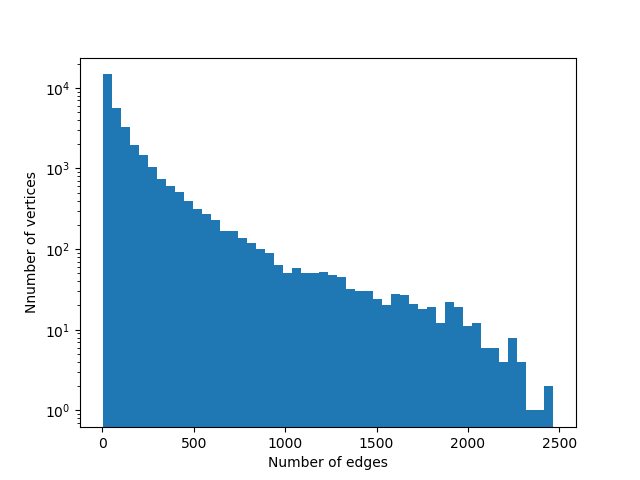
\includegraphics[width=\columnwidth]{../good_plots/degree_distribution_10_mil.png}
	\caption{Degree distribution for a representative graph in our dataset, 
		demonstrating that the graphs we chose are power-law graphs.}
	\label{fig:degree_distribution}
\end{figure}

We selected eleven graphs to analyze. Although we originally chose several 
others, we were limited by the hardware we had the funds to rent to analyzing 
relatively small graphs. A tradeoff exists between the size of a graph, the 
number of workers assigned to handle its vertices, and the amount of memory on 
a server. First, there is a minimum amount of memory that a Giraph worker 
requires in 
order to run. This puts an upper bound on the number of workers that can be run 
on any machine. Second, there appears to be a minimum number of workers that 
can be assigned to a graph of a given size in Giraph: when too few are 
assigned, the job fails. Presumably, this is because each worker can only 
feasibly handle a certain number of vertices, although it is unclear why Giraph 
chooses to terminate jobs rather than allowing them to eventually complete. 
This factor puts a lower bound on the number of workers that can be assigned to 
a graph, which is dependent on the size of the graph. Given these constraints, 
we restricted ourselves to graphs with approximately 200 million edges or fewer.

Our graphs came from the Laboratory for Web Algorithmics (LAW)
\cite{BoVWFI, BRSLLP}. We considered using artificial graphs generated by 
Facebook's Darwini project \cite{edunov_darwini:_2016}, but eventually 
concluded that they were too large. The LAW graphs come 
from a variety of places. We selected a diverse subset of them, as shown in 
Table \ref{tab:graph_types}.

We also paid attention to the distribution of the degrees of the vertices in 
the graphs that we chose. Since most natural graphs are power-law distributed, 
our graphs primarily follow that pattern. Figure \ref{fig:degree_distribution} 
shows a representative example of the degree distribution of a graph in our 
dataset. 

\begin{figure}[!t]
	\centering
	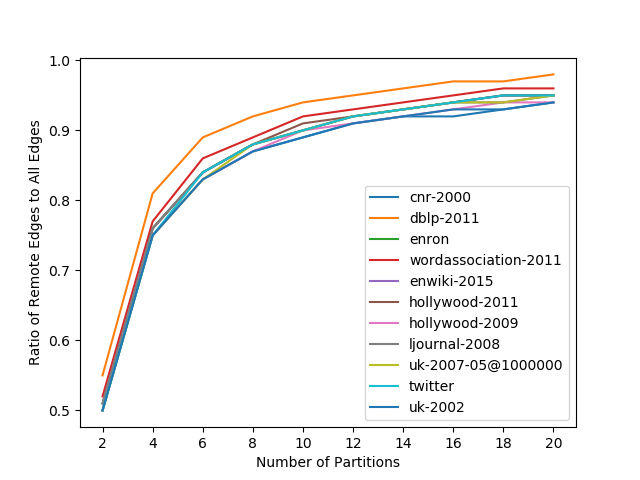
\includegraphics[width=\columnwidth]{../good_plots/remote_to_all_modulo.png}
	\caption{Ratio of remote edges (requiring messages to be sent across the 
	network) to all edges for various numbers of partitions, where partitioning 
	is done by taking the modulus of the vertex ID and number of workers.}
	\label{fig:remote_to_all_mod}
\end{figure}

\begin{figure}[!t]
	\centering
	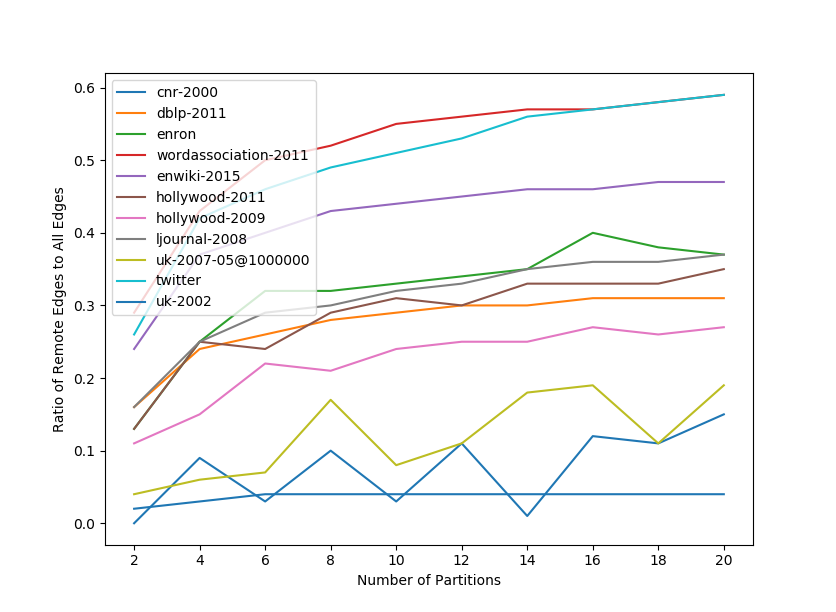
\includegraphics[width=\columnwidth]{../good_plots/remote_to_all_chunked.png}
	\caption{Ratio of remote edges to all edges for various numbers of 
		partitions, where range partitioning is used.}
	\label{fig:remote_to_all_range}
\end{figure}

We ran experiments to look at two metrics that we believe are predictors of 
performance: the number of edges given to each worker that require network 
requests, and the range of the number of edges given to each worker. We chose 
the first metric because we predict that if a worker is assigned a high 
proportion of edges that require it to make network requests, the time taken to 
run each step of computation will be much higher. Recall that in PageRank, 
every computational step requires a message to be sent along every edge. If 
that message begins and ends at vertices that are stored on the same machine, 
the overhead is much lower than it would be if the source and destination 
vertices are stored on two separate machines, thus necessitating a network 
request. Therefore, we measure the ratio between the number of local edges and 
the total edges assigned to a worker for various numbers of partitions and two 
partitioning schemes. Figures \ref{fig:remote_to_all_mod} and 
\ref{fig:remote_to_all_range} show the results.

Figure \ref{fig:remote_to_all_mod} shows the partitioning scheme where vertices 
are assigned to workers by taking the modulo of their vertex ID with the number 
of workers in the cluster. Figure \ref{fig:remote_to_all_range} shows the 
results of ranged partitioning. We hypothesized that both partitioning schemes 
would yield a graph similar to Figure \ref{fig:remote_to_all_mod}, because if 
vertices are truly randomly assigned, then there is a greater chance of a 
vertex being assigned to a remote worker than a local one as the number of 
workers increases. However, range partitioning is not random - it takes 
locality into account. The graphs we analyze are taken from real-world 
data. Since they have to 
be created by some sort of crawler or traversal algorithm, they exhibit a 
certain amount of locality. Range partitioning therefore
does a significantly better job than modulo partitioning at reducing the 
fraction of remote edges to local edges, as shown in Figure 
\ref{fig:remote_to_all_range}.

The second predictor of performance that we measured was the variation of the 
number of edges assigned to each worker. We assigned an equal number of 
vertices to each worker with all of our partitioning schemes, but this did not 
guarantee that the number of edges was the same. To our surprise, large graphs 
tend to approach edge equanimity even with the simple partitioning algorithms 
we use, which make no attempt to assign edges equally. We quantified this 
relationship in terms of the coefficient of variation of the number of edges 
assigned to each worker, for a varied number of workers, as shown in Figures 
\ref{fig:cv_mod} and \ref{fig:cv_range}.

\begin{figure}[!t]
	\centering
	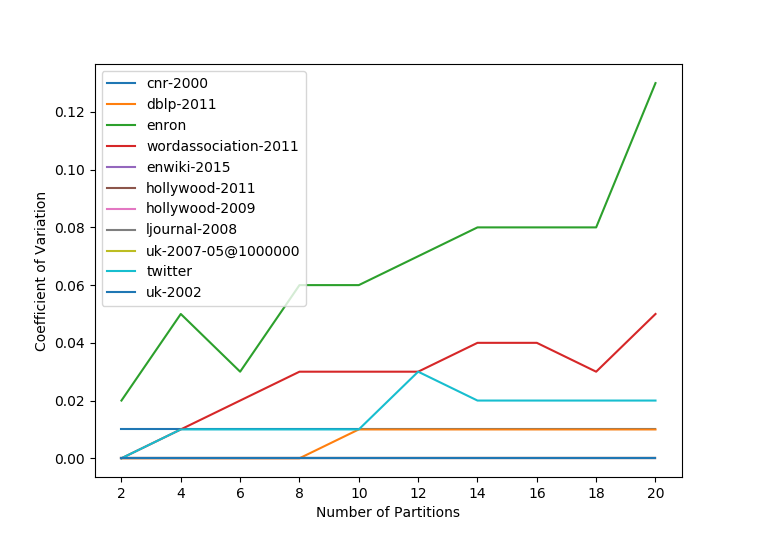
\includegraphics[width=\columnwidth]{../good_plots/range_as_cv_modulo.png}
	\caption{Range of the maximum number of edges handled by each worker to the 
		minimum handled by any worker, expressed by the coefficient of 
		variation, 
		for various numbers of partitions, with modulo partitioning.}
	\label{fig:cv_mod}
\end{figure}

\begin{figure}[!t]
	\centering
	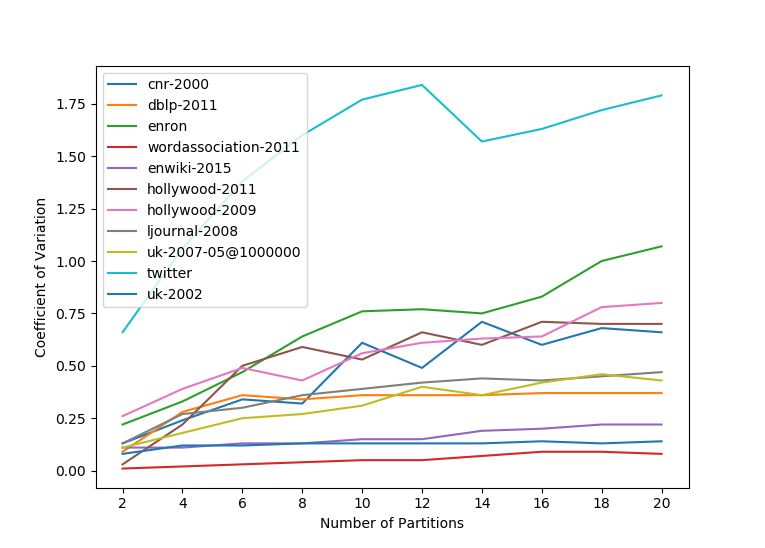
\includegraphics[width=\columnwidth]{../good_plots/range_as_cv_chunked.png}
	\caption{Range of the maximum number of edges handled by each worker to the 
		minimum handled by any worker, expressed by the coefficient of 
		variation, for various numbers of partitions, with range 
		partitioning.}
	\label{fig:cv_range}
\end{figure}

Figure \ref{fig:cv_range} shows that range partitioning led to a significantly 
higher 
difference between the number of edges assigned to each worker. This is likely 
due to locality again - range partitioning tends to capture any clustering 
present in the graph, whereas modulo partitioning evenly distributes clusters 
and breaks them up. One graph in particular stood out from the others: twitter, 
which draws edges between followers on the Twitter social network. Twitter is 
the largest graph we analyze, but large graphs do not necessarily appear to 
correspond to high coefficients of variation when it comes to edge 
distribution. It is possible that the twitter graph has more severe clustering 
than the other graphs, but why it should be so much higher than (for example) 
another social network graph like ljournal-2008, we do not know. Figure 
\ref{fig:cv_mod} shows a lower range of number of edges assigned to each 
worker, perhaps because modulo partitioning is closer to completely random than 
range partitioning. Here, many graphs have such even edge partitioning that 
their coefficient of variation is zero for all numbers of partitions. 

Our takeaway from these experiments is that there is a tradeoff to be made when 
choosing a partitioning algorithm. If a particular job is concerned with having 
workers that lag behind the fastest workers in the cluster, it is probably 
important to choose to distribute edges as well as vertices evenly among the 
workers, and modulo partitioning should be used. If a job is likely to be 
network bound, range partitioning may be more effective, since it leverages 
locality to reduce the number of remote edges each worker must handle.